\documentclass{article}
\usepackage{amsmath, amssymb}
\usepackage{graphicx}
\usepackage{listings}
\usepackage{color}
\usepackage{caption}
\usepackage{geometry}
\geometry{margin=1in}

\definecolor{codegray}{gray}{0.9}
\lstset{
  backgroundcolor=\color{codegray},
  basicstyle=\ttfamily\footnotesize,
  breaklines=true
}

\title{Eigenvector Analysis using Python}
\author{Mahla Entezari}
\date{October 2023}

\begin{document}

\maketitle

\section*{1. Introduction}
This report explores the eigenstructure of a 2x2 matrix using Python. The focus is on calculating eigenvalues and eigenvectors, normalizing them, and visualizing their transformations via matrix multiplication. Such visualization is essential for understanding how linear transformations behave geometrically.

\section*{2. Code Implementation}
The Python code below computes the eigenvalues and eigenvectors of a matrix $A$, normalizes the eigenvectors, and visualizes both the original and transformed vectors.

\subsection*{Python Code}
\begin{lstlisting}
import numpy as np
import matplotlib.pyplot as plt

A = np.array([[1, 2], [3, 4]])
eigenvalues, eigenvectors = np.linalg.eig(A)
eigenvectors = eigenvectors / np.linalg.norm(eigenvectors, axis=0)
Av = np.dot(A, eigenvectors)

plt.quiver([0, 0], [0, 0], eigenvectors[0, :], eigenvectors[1, :], angles='xy', scale_units='xy', scale=1, color=['r', 'b'], label='Normalized Eigenvectors')
plt.quiver([0, 0], [0, 0], Av[0, :], Av[1, :], angles='xy', scale_units='xy', scale=1, color=['g', 'y'], label='Av')
plt.xlim(-10, 10)
plt.ylim(-10, 10)
plt.xlabel('x')
plt.ylabel('y')
plt.title('Normalized Eigenvectors of A and Av')
plt.legend()
plt.grid()
plt.savefig('eigenvectors_plot.png')
plt.show()
\end{lstlisting}

\section*{3. Output and Visualization}
The plot generated by the code visually contrasts the normalized eigenvectors with their transformed counterparts after applying the matrix $A$. This helps illustrate the action of the matrix on its eigenvectors.

\begin{figure}[h!]
    \centering
    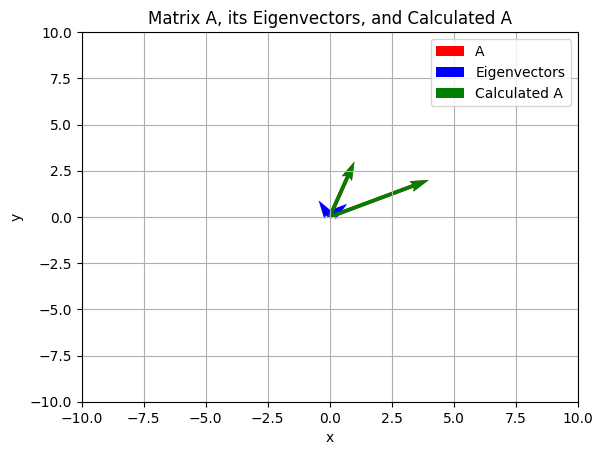
\includegraphics[width=0.7\textwidth]{output.png}
    \caption{Visualization of Normalized Eigenvectors and their Transformations by Matrix $A$}
    \label{fig:eigenvectors}
\end{figure}

\section*{4. Conclusion}
Through numerical computation and graphical visualization, we observe how the eigenvectors of a matrix represent directions that remain invariant under transformation by the matrix, only scaled by their corresponding eigenvalues. Such insights are foundational in linear algebra and its applications.

\end{document}

